\documentclass[graphics]{beamer}

\usepackage{graphicx}
\usepackage{verbatim}
\usepackage{wrapfig}
\useoutertheme{shadow}
%\usecolortheme{orchid}
\usecolortheme{seahorse}


% math commands
\newcommand{\be}{\begin{eqnarray}}
\newcommand{\ee}{\end{eqnarray}}
\newcommand{\beq}{\begin{equation}}
\newcommand{\eeq}{\end{equation}}
\def\simless{\mathbin{\lower 3pt\hbox
      {$\rlap{\raise 5pt\hbox{$\char'074$}}\mathchar"7218$}}}
\def\simgreat{\mathbin{\lower 3pt\hbox
      {$\rlap{\raise 5pt\hbox{$\char'076$}}\mathchar"7218$}}} %> or of order

% variables

\def\toonscale{0.45}
\def\mboxy#1{\mbox{\small #1}}


\begin{comment}
\AtBeginSection[]{
  \frame{
    \frametitle{Outline}
    \tableofcontents[currentsection]
  }
}
\end{comment}

\title{Coherent cosmology: wave effects of FRBs and GWs.
}
%\subtitle{interim update}
\author[U. Pen]{Ue-Li Pen and collaborators
}
\date{December 12, 2023}


\begin{document}

%\section*{Introduction}
\section{Lenses}

\begin{comment}
  \subsection{Outline}

  \frame{
    \frametitle{Outline}
    \tableofcontents
  }
\end{comment}

\frame{\maketitle}


  \frame{
    \frametitle{Gravitational Waves, Fast Radio Bursts}
    \begin{itemize}
        \item Coherent, distant source of radiation
        \item Interference effects under multi-path propagation
        \item potential for diffraction limited measurements
        \item new regime: microlensing by stars (or DM)
        \item nanohertz GWs: breakdown of geometric lensing,
          effervescent images
        \item Kirchoff-Fresnel path integral
         \item Morse index, complex images: measure time delays in weak lensing
    \end{itemize}
  }


  \frame{
    \frametitle{FRBs}
    \begin{itemize}
        \item Coherent, distant source of radiation
        \item Scintillate under multi-path propagation          
        \item sensitive to ns time delay propagating for gigaparsecs
        \item corresponds to strain $h \ll 10^{-26}$: far exceeds LIGO
        \item highly elongated antenna pattern: sensitive to
          longitudinal modes          
    \end{itemize}
  }


  \frame{
\vspace{-0.25in}
    \frametitle{FRB110523}
 

%\hspace{2.5in}
\includegraphics[width=2.5in]{Figures/scint110523.png}
\includegraphics[width=1.75in]{Figures/corr110523.png}

Masui++ 2015, Nature, 528, 523
  }

\frame{

    \frametitle{more precision astrometry}
%\vspace{-0.25in}
\begin{center}
%\hspace{-0.5in}
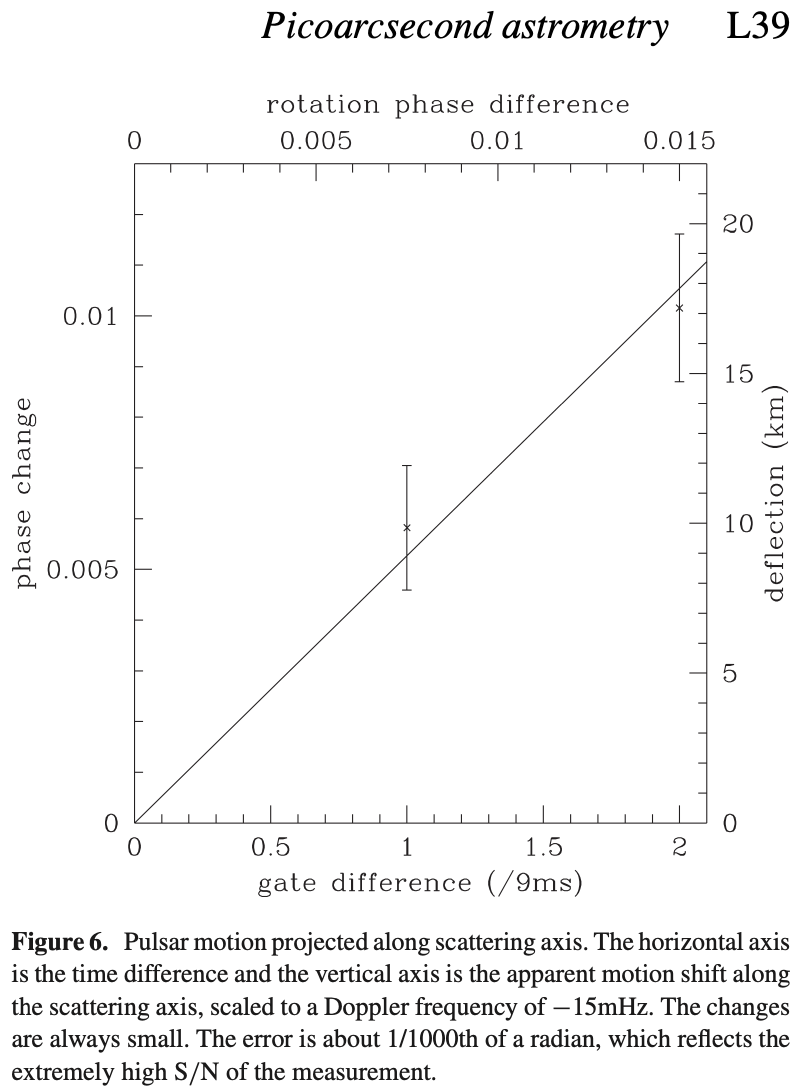
\includegraphics[width=2.05in]{Figures/pico.png}
UP+14
\end{center}
  }



  \frame{
\vspace{-0.5in}
    \frametitle{Wave Microlensing}
    \begin{itemize}
    \item unresolved, echo of voltage stream delayed by microseconds
    \item search voltage stream, or look for scintillation
    \item observables: time delay, flux ratio
    \end{itemize}
  }


  \frame{
\vspace{-0.5in}
    \frametitle{Microlensing: applications}
    \begin{itemize}
    \item DM, stellar mass function, planets
    \item +plasma lensing: direct distance
    \item repeater macrolensing: direct distance
    \end{itemize}
  }

    \frametitle{Current status}

\begin{center}

\includegraphics[width=4.5in]{Figures/leungml.jpg}

Leung++22 (CHIME)
\end{center}
  }
  \frame{
\vspace{-0.5in}
    \frametitle{Microlensing: challenges}
    \begin{itemize}
    \item contamination by plasma in lens galaxy?
    \end{itemize}
  }


  \frame{
\vspace{-0.5in}
    \frametitle{Effervescent Images}
    \begin{itemize}
    \item consider ``rational lens'' potential $\psi(\theta)=\alpha/(1+\theta^2)$
    \item Geometric/eikonal images at $\psi'=\theta$
    \item 5 roots.  1 or 3 real roots, rest imaginary
    \item P-L: at most one imaginary image contributes!
    \item imaginary image can be brighter than unlensed real image
    \end{itemize}
  }


  \frame{
%\vspace{-0.5in}
    \frametitle{Rational 1-D lens}
\begin{center}
\includegraphics[width=3.1in]{Figures/theta-beta.eps}
\end{center}
  }


  \frame{
\vspace{-0.5in}
    \frametitle{New Observables}
    \begin{itemize}
    \item for coherent sources: FRBs, pulsars
    \item weak lensing: imaginary image allows time delay measurement (Jow+21)
    \item strong lensing: delay measurements enable measurement of
      co-linearity (Jow++21)
    \item microlensing: instant time delay, planets (Jow+20)
    \item macrolensing: potentially nano-second delay -- universe
      expands!  Dark energy, etc (Wucknitz+21)
    \item dimensionless strain cm/Gigalightyears $h\sim \Delta t/t \sim 10^{-26}$:
      competitive with LIGO, etc
    \end{itemize}
  }


  \frame{
%\vspace{-0.25in}
    \frametitle{Macro lensing}
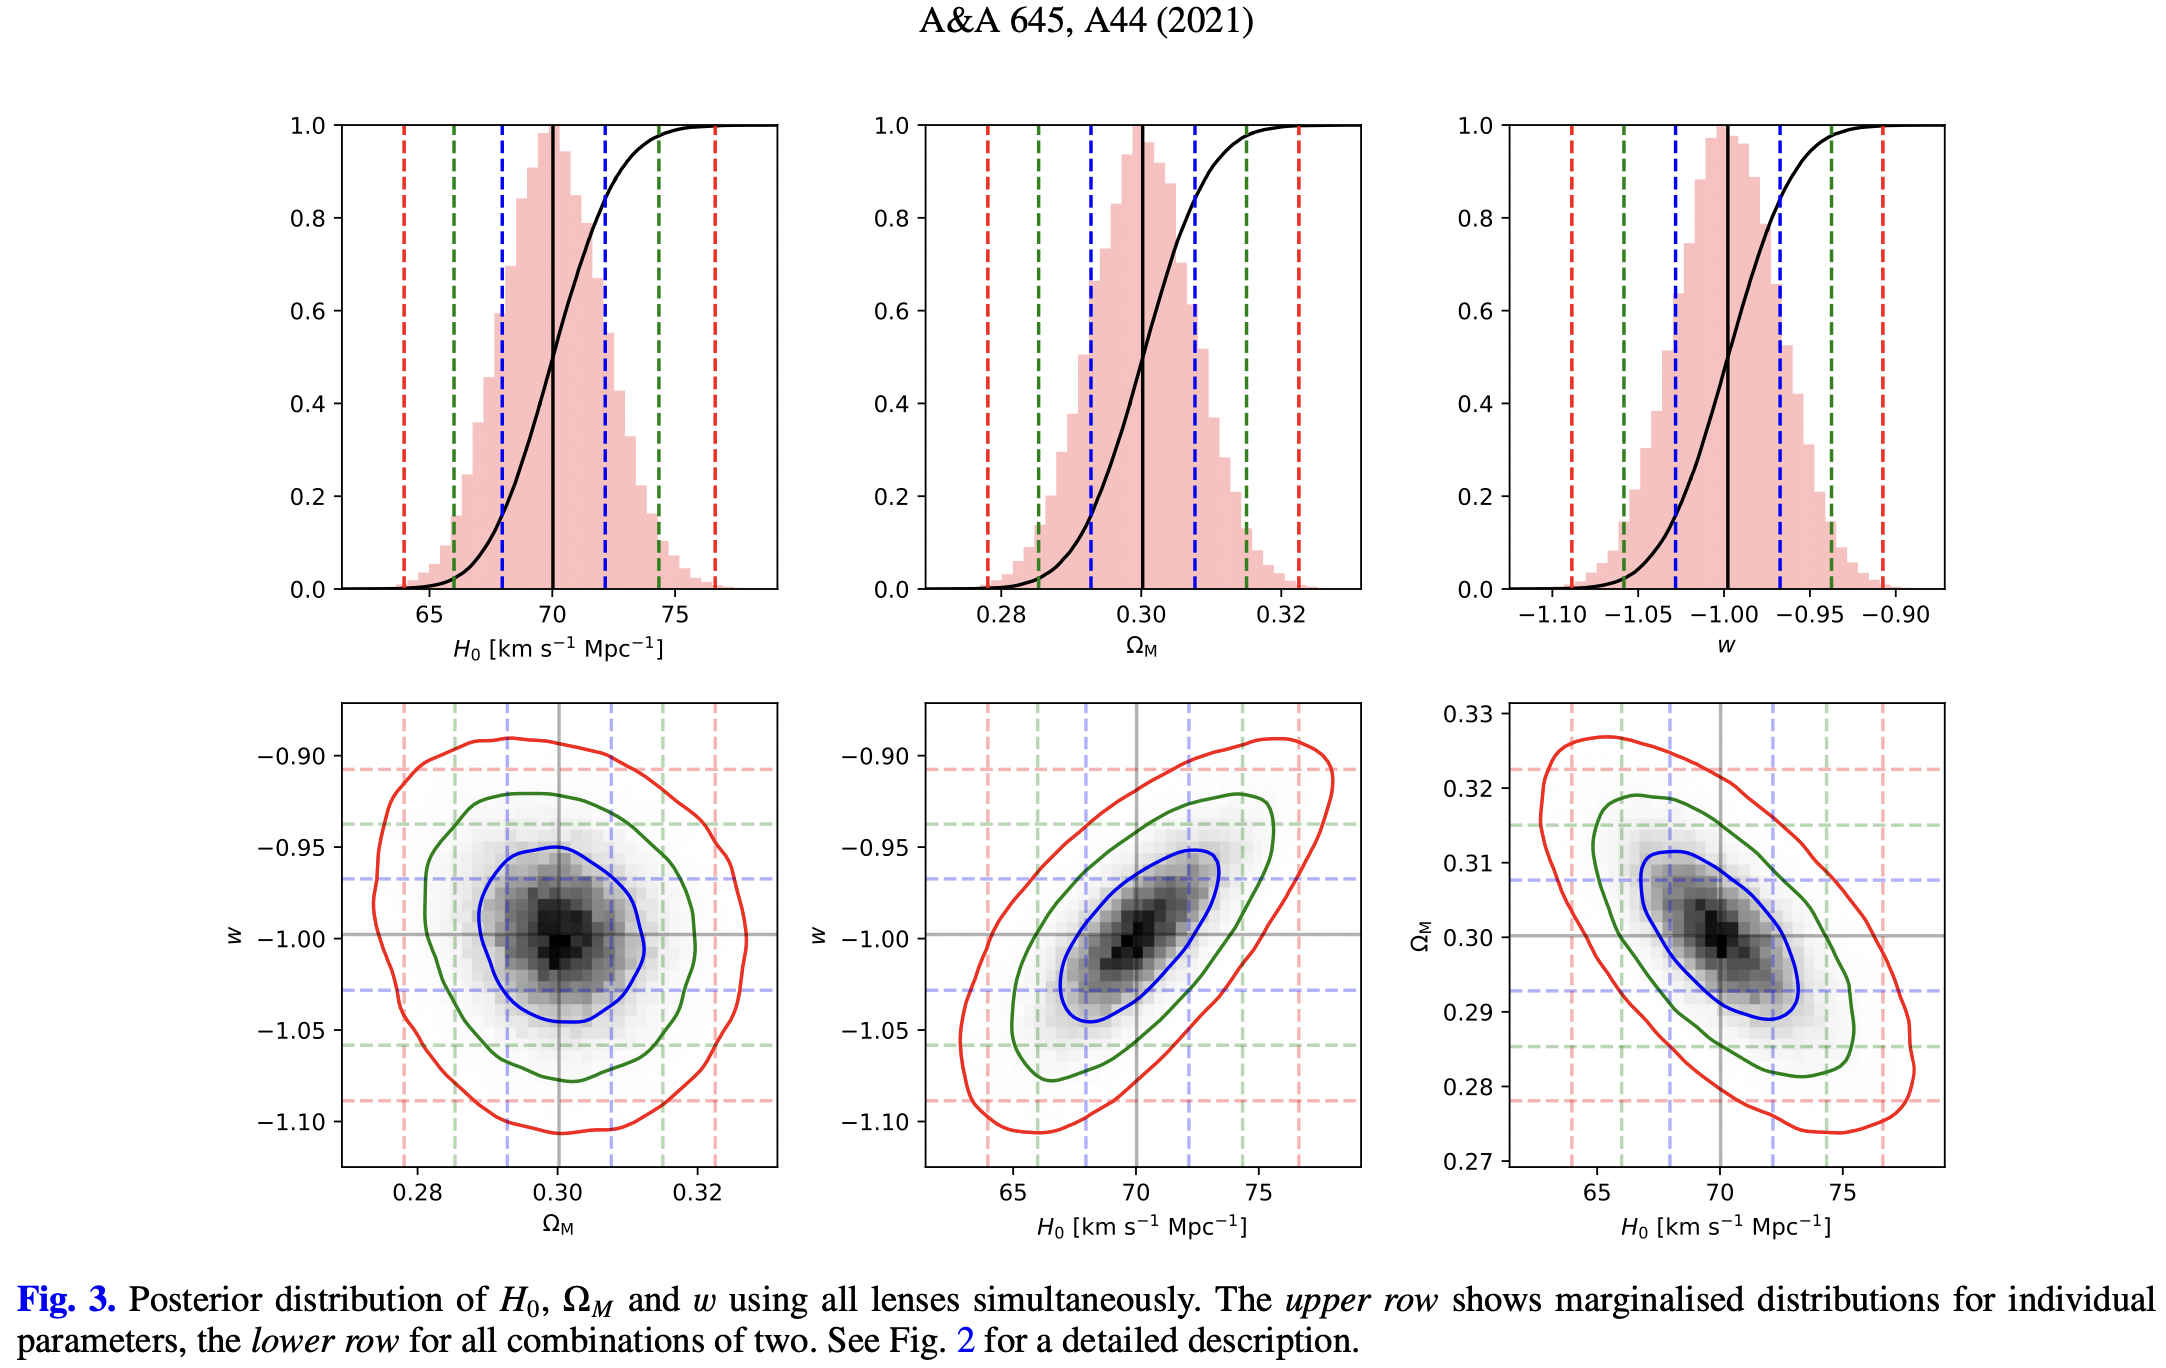
\includegraphics[width=4.5in]{Figures/wucknitz.png}

Wucknitz, Spitler, ULP 2021, A\&A, 645, A44
  }





  \frame{
    \frametitle{Diffractive Gravitational Wave Lensing}
\includegraphics[width=4.5in]{Figures/PTAGWLensing.pdf}

Jow+ in prep
  }


  \frame{
\vspace{-0.5in}
    \frametitle{Discussion}
    \begin{itemize}
    \item Eikonal effects applicable to coherent sources,
      e.g. FRBs, pulsars, LIGO/Lisa GWs
    \item microlensing down to planet size
    \item full wave
effect dominates for long wavelengths as Fresnel scale is bigger then
Einstein radius, i.e. PTA GWs 
    \end{itemize}
  }



  \frame{
%\vspace{-0.5in}
    \frametitle{Conclusions}
    \begin{itemize}
     \item wave optics changes nature of astrophysical observables: Coherent FRB/pulsar/GW      radiation one of the potentially most
      precise measurements in physics
      \item already makes microarcsecond images of pulsars
      \item ISM plasma screens modelled quantitatively as localized
        1-D features, no longer stochastic turbulent volume.
    \item Picard-Lefschetz theory provides alternative interpretation
      of optics, quantum mechanics: imaginary positions and trajectories
      \item next generation FRB telescopes for cosmic mass inventory,
        possibly dark energy/acceleration
      \item PTA weak diffractive lensing may give new tool for Hubble
        Constant tension
    \end{itemize}
  }

\end{document}
